\documentclass{article}
\usepackage{geometry}
\usepackage{flafter}
\geometry{letterpaper, portrait, margin=1in}

\usepackage{hyperref}
\hypersetup{
    colorlinks=true,
    linkcolor=black,
    filecolor=magenta,
    urlcolor=blue,
}

\usepackage{graphicx}
\graphicspath{ {images/} }

\usepackage{tcolorbox}
\usepackage{textcomp}
\usepackage{gensymb}
\usepackage{indentfirst}

\newcommand{\ans}{$\rule{1.5cm}{0.15mm}$}

\title{RoboJackets Firmware Training Week 3 Lab Guide}
\author{Marine Maisonneuve, Logan Schick}
\date{\today\\v1.0}

\begin{document}
\maketitle{}
\setcounter{tocdepth}{2}
\tableofcontents
\pagebreak

%Everything below is for you to edit. Code above sets up the general formatting for the document

\section{Background}
    \subsection{Topics}
        The important topics being discussed this week in lab include datasheets, registers, and Pulse-Width Modulation (PWM).
        
    \subsection{Premise}
        The lab premise is to use a push button change the brightness of a LED. This system will use interrupts to change PWM registers to control the power output.
        
    \subsection{Pulse Width Modulation}
        PWM is a method of generating variable voltage output with a static source. By alternating between a low and high voltage, the average effect of a middle voltage can be achieved. The average output voltage is determined by the value of the "high time" (when the voltage is high) over the total time (the time the voltage is high and low). 
        
        In this case, the source of the high and low voltage is a specific pin and the time it's high and low is controlled by a timer. As seen in lecture, timers use a counter that counts up to a max value to  For Fast PWM (the PWM mode we're using in this lab) the pin is set to a value (either high or low) when the counter is at 0 then the pin is set to the opposite when the timer reaches its max value (255) it then resets to 0 starting the process again. 
        
    \subsection{ATMega328P Microcontroller}
        The Arduino Uno is based on ATMega328P microcontroller which has 3 timer setup controlled using timer registers. We can therefore look at the \href{https://www.sparkfun.com/datasheets/Components/SMD/ATMega328.pdf}{datasheet} for the microcontroller to figure out the values for those control registers. To save a bit of time skip to Section 12-15 (specifically Section 15) which explains the timer you’ll be controlling in the lab. To complete the lab the only required readings are the register descriptions for the timers, but other sections such as modes of operation will give a better understanding of what these timers can do.
        
    \subsection{Simulation}
        If you are using a simulation instead of the hardware, do not worry.  The steps are exactly the same. Go to the TinkerCAD link and you will see the circuit that is a subset of the the hardware. The Arduino you see will be what you use, with the LEDs and buttons replicated as they would be on the actual board.
        \begin{figure}[ht]
            \centering
            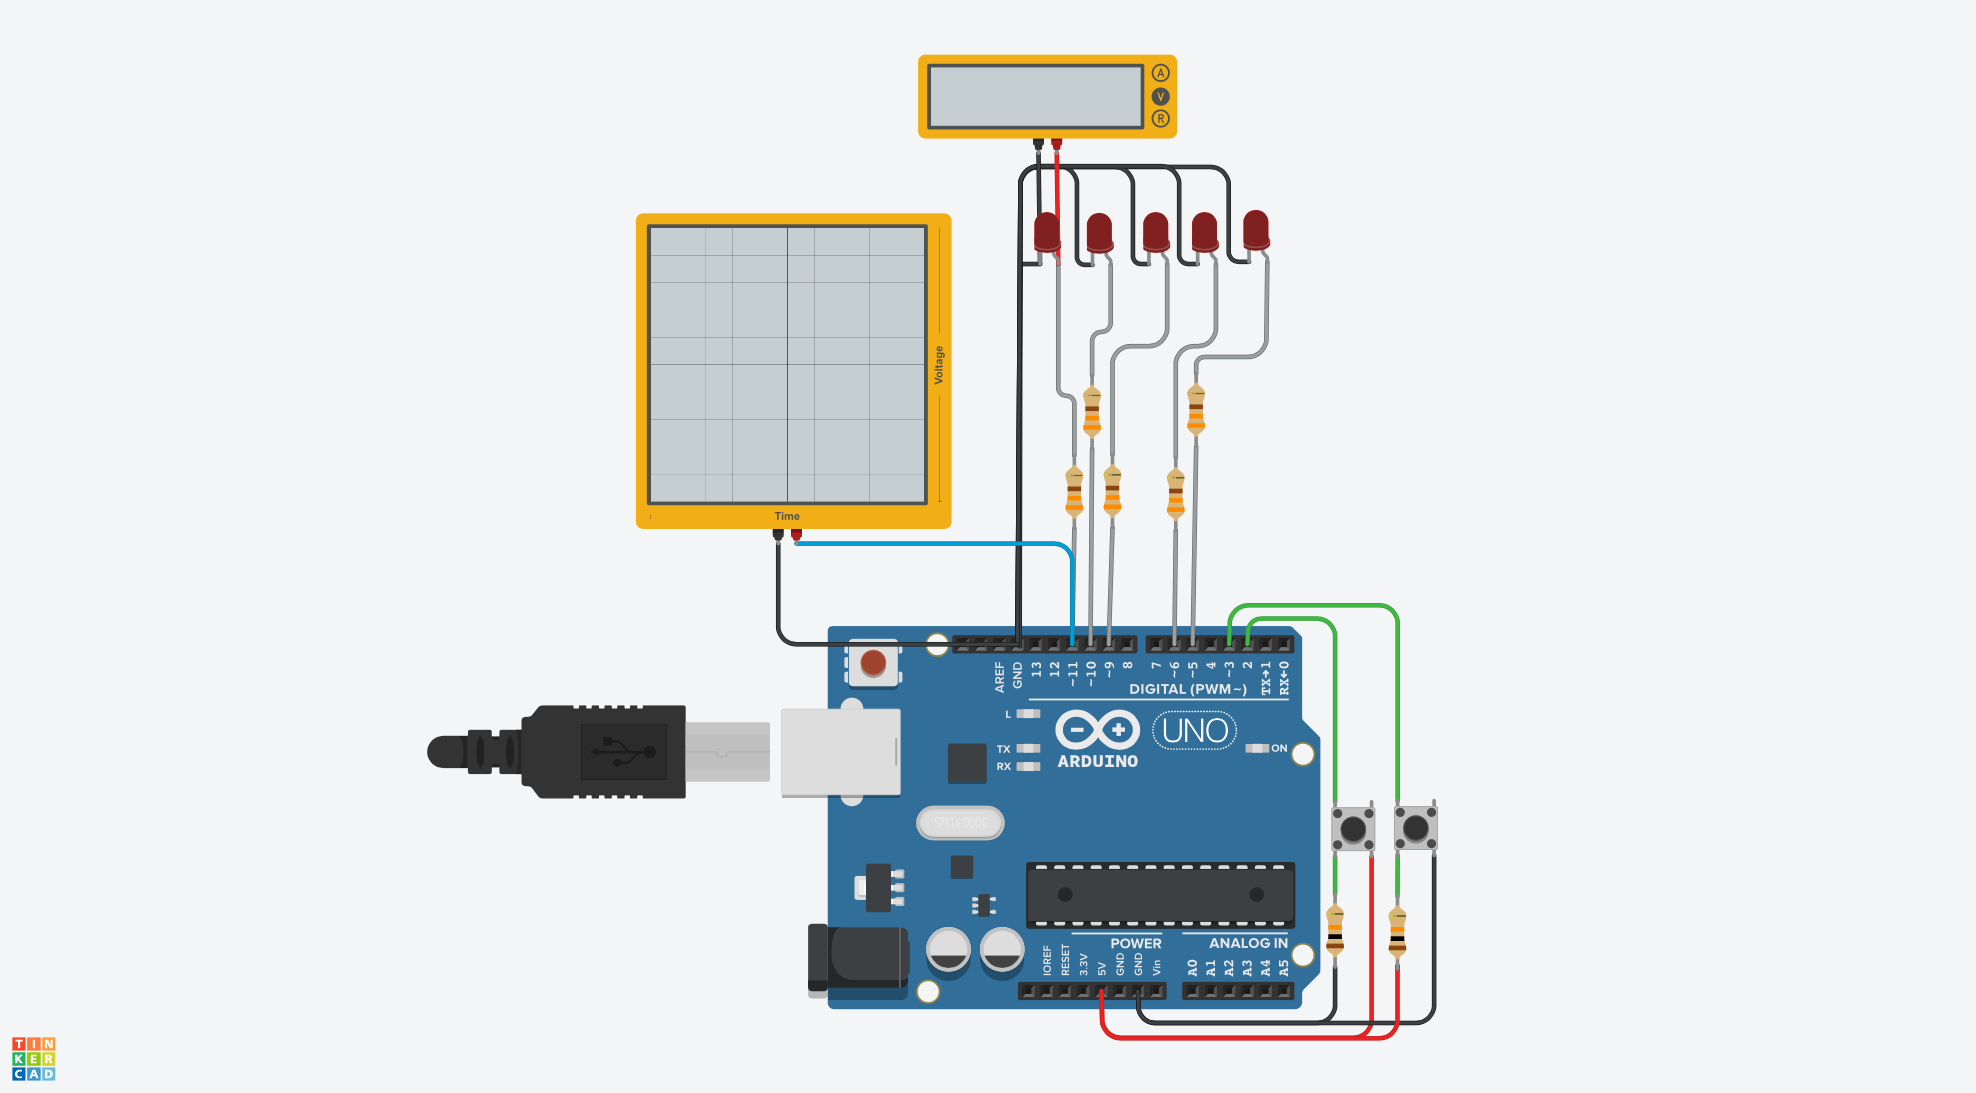
\includegraphics[width = 0.7\textwidth]{images/TinkerCADWires.png}
            \caption{The circuit window of TinkerCAD for this project}
        \end{figure}
        
        \begin{figure}[ht]
            \centering
            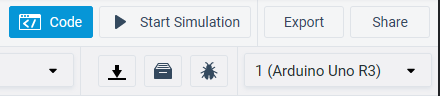
\includegraphics[width = 0.7\textwidth]{images/TinkerCadCode.png}
            \caption{The area which you can use to select your target and compile}
        \end{figure}
        \pagebreak
\section{Materials}
\begin{itemize}
	\item \href{https://www.autodesk.com/education/edu-software/overview}{AutoDesk Education Account}
	\item \href{https://www.tinkercad.com/things/aeAzdEiZjZr}{TinkerCAD}
\end{itemize}
\section{Objectives}
    \subsection{Task 1 - Setup}
        \begin{enumerate}
            \item Use the \href{https://www.sparkfun.com/datasheets/Components/SMD/ATMega328.pdf}{datasheet} section 15 to fill in the empty values in the \texttt{setup()} function.
            \begin{itemize}
                \item You can directly set the values of these specific variables in binary, saving you the need to convert it.
                \item To do that, use the \texttt{0b} notation for the binary values in C++. For example \texttt{int var = 0b101;} sets the value of the variable \texttt{var} to 5.
            \end{itemize}
            \item Fill in TCCR2A value.
            \begin{itemize}
                \item The register description of TCCR2A is given in Section 15.11.1 of the datasheet.
                \item Pin 11 (the pin the led, oscilloscope, and voltmeter are on) is controlled by OC2A which should be put in timer mode Fast PWM mode with the TOP being 0xFF. OC2B can be disconnected. The desired output compare mode of OC2A is either Clear on Compare Match or Set on Compare Match.
                \item For information on setting the output compare mode, refer to Section 15.11.1 Table 15-3.
                \item For information on setting the timer mode refer to Section 15.11.1 Table 15-8. Make sure to read the description of the table above it.
                \item A timing diagram for Fast PWM mode can be found in Section 15.7.3
            \end{itemize}
            \item Fill in TCCR2B value.
            \begin{itemize}
                \item The register description of TCCR2B is given in Section 15.11.2 of the datasheet.
                \item The prescaler value can be set to any as long as the clock isn't stopped. A higher prescaler leads to a lower frequency duty cycle, which will make the wave show up more clearly on the oscilloscope.
                \item For information on setting the prescaler, refer to Section 15.11.2 Table 15-9.
            \end{itemize}
             \item OCR2A is the output compare register which controls when the output compare match triggers.
             \item Composition of OCR2A is in Section 15.11.4.
        \end{enumerate}
    \subsection{Task 2 - Create Interrupt}
        \begin{enumerate}
            \item Have the interrupt method increment the value that goes into the output compare register.
            \begin{itemize}
                \item Note that when using fast PWM the 8 bit output compare register takes in a value from 0 to 255.
                \item Values higher will overflow losing bits above 8, so you may want to account for that.
                \item Set up the interrupt to trigger when the button is pushed.
            \end{itemize}
        \end{enumerate}
        
\section{Troubleshooting}
    \subsection{Solutions}
    We have included the solutions below if you do not complete the lab during the session or if you want to verify your answer. If you need help during the lab ask an instructor!
\begin{itemize}
    \item \href{https://www.tinkercad.com/things/juqsfPwatRF}{TinkerCAD Solution}
    \end{itemize}
\end{document}